\begin{comment}	

The strange math.

\subsection{Backstory}
There was a conflict in russia, where Markow and X had different views an free will. 

Where 
marvo had the position, that random outcomes can be a result of depentend events.

Where X mad the flipped the inference, between:
indepented events $\rightarrow$ random outcomes
Concept of large numbers.

That independence of events are nessary to show the law of large numbers (merky).

Where X mad the flipp, when effects of large numbers are observed, then those mean, indpendenc of events are nessary - for him: free choice.

The senario is, total number of marrages. This percludes free choices, there for the hand of god. Who marrages whom. 

The senario: X observed social zufallsvariablen: yearly total number of mariage and other social statistics.

He observed, that those followed the law of large numbers. We resoned, that that means, that convergence of $\mu$ must mean, that the $X_i$ are indepented. This he set equal to, indiviual made indepente choices.

(Image for the flipped logic)

Inlcude: chapter_Mathematics/Scc001.

---

Marcov showed. That dependent events can produce convergens effects of large numbers.
\end{comment}

\chapter{Markov Chains}

\section{The Law of Large Numbers (LLN)}

The \textbf{Law of Large Numbers (LLN)} is a fundamental theorem in probability theory that describes how averages behave over many repetitions of a random experiment. It ensures that the average of repeated independent observations converges to the expected (theoretical) mean.

\subsection*{Key Symbols}

\begin{center}
\begin{tabular}{ll}
\toprule
\textbf{Symbol} & \textbf{Meaning} \\
\midrule
$X_i$ & Random variable representing the $i$-th trial \\
$\mu = \mathbb{E}[X_i]$ & Expected (mean) value \\
$\overline{X}_n$ & Sample mean after $n$ observations \\
$\xrightarrow{P}$ & Convergence in probability \\
$\xrightarrow{\text{a.s.}}$ & Almost sure convergence \\
\bottomrule
\end{tabular}
\end{center}=

\subsection*{Setup}

Let
\[
\{X_1, X_2, \dots\}
\]
be a sequence of independent and identically distributed (i.i.d.) random variables with finite expected value
\[
\mathbb{E}[X_i] = \mu.
\]

Define the sample mean:
\[
\overline{X}_n = \frac{1}{n} \sum_{i=1}^{n} X_i.
\]

\subsection*{Weak Law of Large Numbers (WLLN)}

The sample mean converges to the expected value \emph{in probability}:
\[
\overline{X}_n \xrightarrow{P} \mu \quad \text{as } n \to \infty,
\]
that is, for every $\varepsilon > 0$,
\[
\lim_{n \to \infty} \mathbb{P}(|\overline{X}_n - \mu| > \varepsilon) = 0.
\]

\subsection*{Strong Law of Large Numbers (SLLN)}

The sample mean converges to $\mu$ \emph{almost surely}:
\[
\overline{X}_n \xrightarrow{\text{a.s.}} \mu \quad \text{as } n \to \infty,
\]
meaning
\[
\mathbb{P}\left( \lim_{n \to \infty} \overline{X}_n = \mu \right) = 1.
\]

\subsection*{Interpretation}

The LLN justifies the use of empirical averages to estimate theoretical expectations. As the number of samples grows, randomness averages out, and the observed mean stabilizes around the true mean.



% ----------------------------------------------------------
\section{Markov Chains and Dependence}

\subsection*{Overview}

\begin{center}
\begin{tabular}{llll}
\toprule
\textbf{Case} & \textbf{Independence} & \textbf{Expectation} & \textbf{LLN Holds?} \\
\midrule
i.i.d. & Yes & Constant ($\mu$) & Yes \\
Stationary Markov Chain & No & Constant ($\mu$) & Yes \\
Ergodic Markov Chain & No & Converges to $\mu$ & Yes \\
\bottomrule
\end{tabular}
\end{center}]

\subsection*{Key Symbols}

\begin{center}
\begin{tabular}{ll}
\toprule
\textbf{Symbol} & \textbf{Meaning} \\
\midrule
Markov property & $\,\mathbb{P}(X_{n+1}\!\mid X_n,\dots)=\mathbb{P}(X_{n+1}\!\mid X_n)$ (local forgetting) \\
Ergodicity & Global forgetting; convergence to a unique $\boldsymbol{\pi}$ \\
$\boldsymbol{\pi}$ & Stationary distribution ($\boldsymbol{\pi}P=\boldsymbol{\pi}$) \\
$S = \{s_1, \dots, s_k\}$ & Finite set of possible states \\
$X_n$ & State of the process at step $n$ \\
$\mathbb{P}(X_{n+1}=s_j \mid X_n=s_i)$ & Transition probability \\
\bottomrule
\end{tabular}
\end{center}


\subsection*{Definition}

A \textbf{Markov chain} is a sequence of random variables
\[
X_1, X_2, X_3, \dots
\]
taking values in a state space
\[
S = \{ s_1, s_2, \dots, s_k \},
\]
and satisfying the \emph{Markov property}:
\[
\mathbb{P}(X_{n+1} = s_j \mid X_n = s_i, X_{n-1}, \dots, X_1)
= \mathbb{P}(X_{n+1} = s_j \mid X_n = s_i),
\quad \forall i,j.
\]

\subsection*{Interpretation Definition}

The \emph{Markov property} is a local forgetting statement: conditional on the
present state, the future is independent of the past. By itself, this property
does \emph{not} imply convergence of empirical averages.\\ 

However, if a Markov chain satisfies additional regularity conditions that
force \emph{global forgetting} (ergodicity)—for example, on a finite state space:
irreducibility, aperiodicity, and positive recurrence—then the chain admits a
unique stationary distribution $\boldsymbol{\pi}$, the law of $X_n$ converges to
$\boldsymbol{\pi}$ regardless of the start, and a Law of Large Numbers holds
for functions of the chain.

\subsection*{Interpretation (General)}

Markov showed that independence is \emph{not necessary} for the Law of Large Numbers
to hold.  Even when consecutive events are dependent---as in a Markov chain---the
average value still converges to a stable limit if the dependence is sufficiently
regular (e.g., the chain is stationary or ergodic).  Thus, the LLN can be
``caused by dependent events.''


\noindent
In particular, independence of the $X_i$ is not necessary for an LLN:
what is needed is sufficient mixing/forgetting of the initial state, as
guaranteed by ergodicity.





% ----------------------------------------------------------
\section{The Idea of Forgetting}

\subsection*{Key Symbols}

\begin{center}
\begin{tabular}{ll}
\toprule
\textbf{Symbol} & \textbf{Meaning} \\
\midrule
$P_{ij}$ & Probability of moving from state $s_i$ to $s_j$ \\
$\pi_j$ & Long-run (stationary) probability of state $s_j$ \\
$\boldsymbol{\pi}$ & Stationary distribution vector \\
Ergodic chain & Chain that “forgets” its start and converges to $\pi$ \\
\bottomrule
\end{tabular}
\end{center}

\subsection*{Local Forgetting}

The \textbf{Markov property} expresses local forgetting:
\[
\mathbb{P}(X_{n+1} = x_{n+1} \mid X_yn = x_n, X_{n-1}, \dots)
= \mathbb{P}(X_{n+1} = x_{n+1} \mid X_n = x_n).
\]
Once the current state is known, the past is irrelevant.

\subsection*{Global Forgetting (Ergodicity)}

In many chains, as $n \to \infty$, the effect of the initial state vanishes:
\[
\lim_{n \to \infty} \mathbb{P}(X_n = s_j \mid X_0 = s_i) = \pi_j,
\]
where $\boldsymbol{\pi} = (\pi_1, \dots, \pi_k)$ is the \emph{stationary distribution}, independent of the start.



% ----------------------------------------------------------
\section{Transition Probabilities and Stationarity}

\subsection*{Key Symbols}

\begin{center}
\begin{tabular}{ll}
\toprule
\textbf{Symbol} & \textbf{Meaning} \\
\midrule
$P_{ij}$ & One-step transition probability \\
$P$ & Transition matrix \\
$\boldsymbol{\pi}^{(n)}$ & Distribution at step $n$ \\
$\boldsymbol{\pi}$ & Stationary distribution \\
$\mu$ & Expected value under stationarity \\
\bottomrule
\end{tabular}
\end{center}

\subsection*{Transition Matrix}

The one-step transition probabilities are collected into a matrix:
\[
P =
\begin{bmatrix}
P_{11} & P_{12} & \cdots & P_{1k} \\
P_{21} & P_{22} & \cdots & P_{2k} \\
\vdots & \vdots & \ddots & \vdots \\
P_{k1} & P_{k2} & \cdots & P_{kk}
\end{bmatrix}, \quad
\sum_{j=1}^{k} P_{ij} = 1.
\]




\subsection*{Stationary Chains}

A chain is \textbf{stationary} if its distribution does not change with time:
\[
\mathbb{P}(X_{n+1} = j) = \mathbb{P}(X_n = j) \quad \forall n.
\]
Then,
\[
\mathbb{E}[X_n] = \mu, \quad
\frac{1}{n}\sum_{i=1}^{n} X_i \xrightarrow{\text{a.s.}} \mu.
\]

\subsection*{Ergodic Chains}

Even if the initial distribution is non-stationary, an \textbf{ergodic} chain converges to a unique stationary distribution:
\[
\boldsymbol{\pi}^{(n)} = \boldsymbol{\pi}^{(0)} P^n \to \boldsymbol{\pi}.
\]
Thus, the Law of Large Numbers still holds:
\[
\frac{1}{n} \sum_{i=1}^{n} X_i \xrightarrow{\text{a.s.}} \mu.
\]


\begin{center}
\begin{tabular}{llll}
\toprule
\textbf{Case} & \textbf{Independence} & \textbf{Expectation} & \textbf{LLN Holds?} \\
\midrule
i.i.d. & Yes & Constant ($\mu$) & Yes \\
Stationary Markov Chain & No & Constant ($\mu$) & Yes \\
Ergodic Markov Chain & No & Converges to $\mu$ & Yes \\
\bottomrule
\end{tabular}
\end{center}



% ----------------------------------------------------------
\section{Example: Two-State Markov Chain}

\subsection*{Key Symbols}

\begin{center}
\begin{tabular}{ll}
\toprule
\textbf{Symbol} & \textbf{Meaning} \\
\midrule
$p_{VV}, p_{VC}, p_{CV}, p_{CC}$ & Transition probabilities \\
$\pi_V, \pi_C$ & Stationary probabilities \\
$\boldsymbol{\pi}^{(0)}$ & Initial distribution \\
$P^n$ & $n$-step transition matrix \\
\bottomrule
\end{tabular}
\end{center}


\subsection*{Setup}

\[
S = \{V, C\}, \quad
P =
\begin{bmatrix}
p_{VV} & p_{VC} \\
p_{CV} & p_{CC}
\end{bmatrix},
\quad
p_{VC} = 1 - p_{VV}, \quad
p_{CV} = 1 - p_{CC}.
\]

The stationary distribution $\boldsymbol{\pi} = [\pi_V, \pi_C]$ satisfies:
\[
\boldsymbol{\pi} P = \boldsymbol{\pi}, \quad \pi_V + \pi_C = 1.
\]

\begin{figure}[htbp]
\centering
\begin{tikzpicture}[
    scale=1.2,
    transform shape,
    ->, >=Stealth,
    node distance=2cm,
    font=\large,
    every edge/.style={draw, thick, black}
]

% Define node styles
\tikzset{
    vowel/.style={
        circle,
        draw=orange!90!black,
        very thick,
        minimum size=1cm,
        text=orange!90!black,
        font=\bfseries\Large,
        align=center
    },
    consonant/.style={
        circle,
        draw=blue!80!black,
        very thick,
        minimum size=1cm,
        text=blue!80!black,
        font=\bfseries\Large,
        align=center
    }
}

% Nodes
\node[vowel] (V) {V};
\node[consonant, right of=V] (C) {C};

% Self-loops
\path (V) edge[loop left, min distance=10mm, in=210, out=150]
    node[left=3pt] {$p_{VV}= 0.13$} (V);
\path (C) edge[loop right, min distance=10mm, in=30, out=-30]
    node[right=3pt] {$p_{CC}= 0.33$} (C);

% Cross transitions
\path (V) edge[bend left=90] node[above] {$p_{VC}= 0.87$} (C);
\path (C) edge[bend left=90] node[below] {$p_{CV}= 0.67$} (V);

\end{tikzpicture}
\caption{Vowel–Consonant Transition Diagram}
\label{fig:vowel-consonant-diagram}
\end{figure}
=
\subsection*{Example}

Two-state system:
\[
S = \{V, C\}, \quad
P =
\begin{bmatrix}
0.8 & 0.2 \\
0.4 & 0.6
\end{bmatrix}.
\]
The probability of transitioning depends only on the current state—how we got there is irrelevant.



\subsection*{Example Values}

\[
P =
\begin{bmatrix}
0.8 & 0.2 \\
0.4 & 0.6
\end{bmatrix}
\Rightarrow
\boldsymbol{\pi} = [0.667, 0.333].
\]

Thus, vowels occur about $2/3$ of the time, consonants $1/3$, regardless of the starting state.

\subsection*{Interpretation}

This model can represent alternation between vowels and consonants in random text generation.  
Even though events are dependent, the LLN still applies—the long-run proportion of vowels stabilizes at the stationary distribution.


% ----------------------------------------------------------
\section{Evolution and Convergence}

\subsection*{Evolution Equation}

The evolution of state probabilities is governed by:
\[
\boldsymbol{\pi}^{(n+1)} = \boldsymbol{\pi}^{(n)} P, \quad
\boldsymbol{\pi}^{(n)} = \boldsymbol{\pi}^{(0)} P^n.
\]

Different initial distributions (e.g., all vowels, all consonants, or mixed) will all converge to the same stationary distribution in ergodic chains.

\subsection*{Visualization}

A plot of $\pi_V^{(n)}$ vs. $n$ shows convergence toward the equilibrium $\pi_V = 0.667$ for all initial conditions—illustrating the \emph{forgetting property} of Markov chains.

\subsection*{Key Symbols}

\begin{center}
\begin{tabular}{ll}
\toprule
\textbf{Symbol} & \textbf{Meaning} \\
\midrule
$\boldsymbol{\pi}^{(0)}$ & Initial distribution vector \\
$\boldsymbol{\pi}^{(n)}$ & Distribution after $n$ steps \\
$P^n$ & $n$-step transition probabilities \\
Stationary $\boldsymbol{\pi}$ & Limiting equilibrium distribution \\
\bottomrule
\end{tabular}
\end{center}

\bigskip

\noindent
\textbf{Final Takeaway:}  
The Law of Large Numbers extends naturally to dependent sequences like Markov chains.  
Even when each step depends on the last, as long as the chain is stationary or ergodic, empirical averages still converge to theoretical expectations.  
The process may “forget” its past, but its long-run behavior remains predictable.

\chapter{Markov Chains}


\section*{The Markov Chain Case}

\subsection*{Definition}

A \textbf{Markov chain} is a sequence of random variables

\begin{align}
X_1, X_2, X_3, \dots
\end{align}

taking values in a state space \( S = \{ s_1, s_2, \dots, s_k \} \)
and satisfying the \emph{Markov property}:

\begin{align}
\mathbb{P}(X_{n+1} = s_j \mid X_n = s_i, X_{n-1}, \dots, X_1)
= \mathbb{P}(X_{n+1} = s_j \mid X_n = s_i)
\quad \forall i, j.
\end{align}




\section*{The Idea of Forgetting}

The essential feature of a Markov chain is the \emph{Markov property}:
\[
\mathbb{P}(X_{n+1} = x_{n+1} \mid X_n = x_n, X_{n-1}, \dots, X_1)
= \mathbb{P}(X_{n+1} = x_{n+1} \mid X_n = x_n).
\]
This means that the conditional probability distribution of the next state $X_{n+1}$ 
depends only on the present state $X_n$, and not on any of the previous states 
$X_{n-1}, \dots, X_1$. 

In other words, the process \emph{forgets} its past once the current state is known. 
Knowing how the system arrived at $X_n$ does not provide any additional information 
about its future beyond what is already contained in the current state. 

\subsection*{Forgetting in the Long Run}

Although the Markov property is a local form of forgetting (the next step depends 
only on the present), many Markov chains also exhibit \emph{global forgetting}: 
the influence of the initial state disappears as $n \to \infty$. 

For an ergodic Markov chain,
\[
\lim_{n \to \infty} \mathbb{P}(X_n = s_j \mid X_0 = s_i) = \pi_j,
\]
where $\pi$ is the stationary distribution independent of the starting state $s_i$.
This means that the system eventually reaches a steady behavior and ``forgets'' 
where it	=

\subsection*{Conceptual Example}

Consider a simple two-state system:
\[
S = \{V, C\},
\]
where $V$ represents a vowel and $C$ a consonant. The transitions are given by
\[
\mathbb{P}(X_{n+1}=V \mid X_n=V) = 0.8, \quad
\mathbb{P}(X_{n+1}=C \mid X_n=V) = 0.2,
\]
\[
\mathbb{P}(X_{n+1}=V \mid X_n=C) = 0.4, \quad
\mathbb{P}(X_{n+1}=C \mid X_n=C) = 0.6.
\]

If the current state is a vowel ($X_n = V$), the probability of the next state being 
a vowel is always $0.8$, no matter how we reached the current vowel. Whether the 
previous sequence was ``CVCV'' or ``VVVV'' does not change the probability of the 
next step. Thus, only the \emph{current state} matters for predicting the next one.



\subsection{Transiition probablity}



The transition probabilities are given by
\[
P_{ij} = \mathbb{P}(X_{n+1} = s_j \mid X_n = s_i),
\]
and can be arranged into a matrix:
\[
P =
\begin{bmatrix}
P_{11} & P_{12} & \cdots & P_{1k} \\
P_{21} & P_{22} & \cdots & P_{2k} \\
\vdots & \vdots & \ddots & \vdots \\
P_{k1} & P_{k2} & \cdots & P_{kk}
\end{bmatrix}, \quad
\sum_{j=1}^{k} P_{ij} = 1.
\]



\subsection*{Stationary and Ergodic Chains}

A Markov chain is said to be \textbf{stationary} if its distribution does not
change with time:
\[
\mathbb{P}(X_{n+1} = j) = \mathbb{P}(X_n = j) \quad \forall n.
\]
In this case,
\[
\mathbb{E}[X_n] = \mathbb{E}[X_1] = \mu,
\]
and the Law of Large Numbers holds even though the $X_i$ are dependent:
\[
\frac{1}{n} \sum_{i=1}^{n} X_i \xrightarrow{\text{a.s.}} \mu.
\]

If the chain is not stationary but is \textbf{ergodic} (meaning it forgets its
initial state and converges to a unique stationary distribution), then
\[
\mathbb{E}[X_i] \to \mu \quad \text{as } i \to \infty,
\]
and the sample average still satisfies
\[
\frac{1}{n} \sum_{i=1}^{n} X_i \xrightarrow{\text{a.s.}} \mu.
\]

\subsection*{Summary}

\begin{center}
\begin{tabular}{@{}llll@{}}
\toprule
\textbf{Case} & \textbf{Independence} & \textbf{Expectations} & \textbf{LLN holds?} \\
\midrule
i.i.d. & Yes & All equal ($\mathbb{E}[X_i] = \mu$) & Yes \\
Markov chain (stationary) & No & All equal ($\mathbb{E}[X_i] = \mu$) & Yes \\
Markov chain (ergodic, non-stationary start) & No & Different initially, converge to $\mu$ & Yes \\
\bottomrule
\end{tabular}
\end{center}




Let>
\section*{3. Example: Two-State Markov Chain (Vowel--Consonant)}

Consider a system with two states:
\[
S = \{ V, C \},
\]
representing ``Vowel'' and ``Consonant.''  
The transition probabilities are:

\[
P =
\begin{bmatrix}
p_{VV} & p_{VC} \\
p_{CV} & p_{CC}
\end{bmatrix},
\quad
p_{VC} = 1 - p_{VV}, \quad
p_{CV} = 1 - p_{CC}.
\]

The stationary distribution \( \boldsymbol{\pi} = [\pi_V, \pi_C] \) satisfies:
\[
\begin{cases}
\pi_V = \pi_V p_{VV} + \pi_C p_{CV}, \\
\pi_C = \pi_V p_{VC} + \pi_C p_{CC}, \\
\pi_V + \pi_C = 1.
\end{cases}
\]


\section*{4. TikZ Diagram Representation}

\begin{figure}[htbp]
\centering
\begin{tikzpicture}[
    scale=1.2,
    transform shape,
    ->, >=Stealth,
    node distance=2cm,
    font=\large,
    every edge/.style={draw, thick, black}
]

% Define node styles
\tikzset{
    vowel/.style={
        circle,
        draw=orange!90!black,
        very thick,
        minimum size=1cm,
        text=orange!90!black,
        font=\bfseries\Large,
        align=center
    },
    consonant/.style={
        circle,
        draw=blue!80!black,
        very thick,
        minimum size=1cm,
        text=blue!80!black,
        font=\bfseries\Large,
        align=center
    }
}

% Nodes
\node[vowel] (V) {V};
\node[consonant, right of=V] (C) {C};

% Self-loops
\path (V) edge[loop left, min distance=10mm, in=210, out=150]
    node[left=3pt] {$p_{VV}= 0.13$} (V);
\path (C) edge[loop right, min distance=10mm, in=30, out=-30]
    node[right=3pt] {$p_{CC}= 0.33$} (C);

% Cross transitions
\path (V) edge[bend left=90] node[above] {$p_{VC}= 0.87$} (C);
\path (C) edge[bend left=90] node[below] {$p_{CV}= 0.67$} (V);

\end{tikzpicture}
\caption{Vowel–Consonant Transition Diagram}
\label{fig:vowel-consonant-diagram}
\end{figure}


\section*{5. Interpretation}

This two-state Markov chain models how a process (such as forming random words)
may alternate between vowels and consonants.
Even though the events are dependent,
if the chain is stationary or ergodic,
the Law of Large Numbers still holds:
\[
\frac{1}{n} \sum_{i=1}^{n} X_i \xrightarrow{\text{a.s.}} \mathbb{E}[X_1].
\]



\section*{Evolution of a Markov Chain and Initial Conditions}

\subsection*{Probability Distribution Over Time}

For a Markov chain with state space 
\[
S = \{s_1, s_2, \dots, s_k\},
\]
the probabilities of being in each state at time $n$ are collected in a row vector:
\[
\boldsymbol{\pi}^{(n)} =
\begin{bmatrix}
\mathbb{P}(X_n = s_1) &
\mathbb{P}(X_n = s_2) &
\cdots &
\mathbb{P}(X_n = s_k)
\end{bmatrix}.
\]

The evolution of the chain is governed by the \emph{transition matrix} $P$, where
\[
P_{ij} = \mathbb{P}(X_{n+1} = s_j \mid X_n = s_i),
\]
and each row sums to 1.  

The distribution at the next time step is given by
\[
\boldsymbol{\pi}^{(n+1)} = \boldsymbol{\pi}^{(n)} P,
\]
which means that the probabilities at time $n+1$ are obtained by multiplying
the current probabilities by the transition matrix.  
By repeated application,
\[
\boldsymbol{\pi}^{(n)} = \boldsymbol{\pi}^{(0)} P^n.
\]

\subsection*{Example: Two-State Chain (Vowels and Consonants)}

Let
\[
P =
\begin{bmatrix}
0.8 & 0.2 \\
0.4 & 0.6
\end{bmatrix},
\quad S = \{V, C\}.
\]
This means:
\begin{itemize}
    \item If currently a vowel ($V$), the next is vowel with probability $0.8$, consonant with $0.2$.
    \item If currently a consonant ($C$), the next is vowel with probability $0.4$, consonant with $0.6$.
\end{itemize}

\subsection*{Different Initial Distributions}

The initial vector $\boldsymbol{\pi}^{(0)}$ represents the probabilities of starting in each state.  
It can be any valid probability distribution (summing to 1), for example:

\begin{center}
\begin{tabular}{@{}lll@{}}
\toprule
\textbf{Starting condition} & \textbf{Initial vector $\boldsymbol{\pi}^{(0)}$} & \textbf{Meaning} \\ \midrule
All vowels & $[1,\, 0]$ & Certain start in $V$ \\
All consonants & $[0,\, 1]$ & Certain start in $C$ \\
Half vowels, half consonants & $[0.5,\, 0.5]$ & Mixed random start \\
30\% vowels, 70\% consonants & $[0.3,\, 0.7]$ & Biased random start \\
\bottomrule
\end{tabular}
\end{center}

Each of these starting distributions evolves over time according to
\[
\boldsymbol{\pi}^{(n)} = \boldsymbol{\pi}^{(0)} P^n.
\]

For example:
\[
\begin{aligned}
\text{If } \boldsymbol{\pi}^{(0)} &= [1, 0], & \boldsymbol{\pi}^{(1)} &= [0.8, 0.2], & \boldsymbol{\pi}^{(2)} &= [0.72, 0.28], \\
\text{If } \boldsymbol{\pi}^{(0)} &= [0, 1], & \boldsymbol{\pi}^{(1)} &= [0.4, 0.6], & \boldsymbol{\pi}^{(2)} &= [0.56, 0.44].
\end{aligned}
\]

Although they start differently, both sequences converge to the same long-run equilibrium.

\subsection*{Stationary Distribution}

A \textbf{stationary distribution} $\boldsymbol{\pi}$ is one that remains unchanged after multiplication by $P$:
\[
\boldsymbol{\pi} P = \boldsymbol{\pi}, \qquad \sum_i \pi_i = 1.
\]
It represents the equilibrium probabilities of being in each state.

For the matrix above,
\[
\boldsymbol{\pi} = [0.667, 0.333].
\]
That means that, in the long run, the process will be in vowels about 66.7\% of the time and in consonants about 33.3\% of the time.

\subsection*{Visualization of Convergence (``Forgetting'')}

\begin{center}
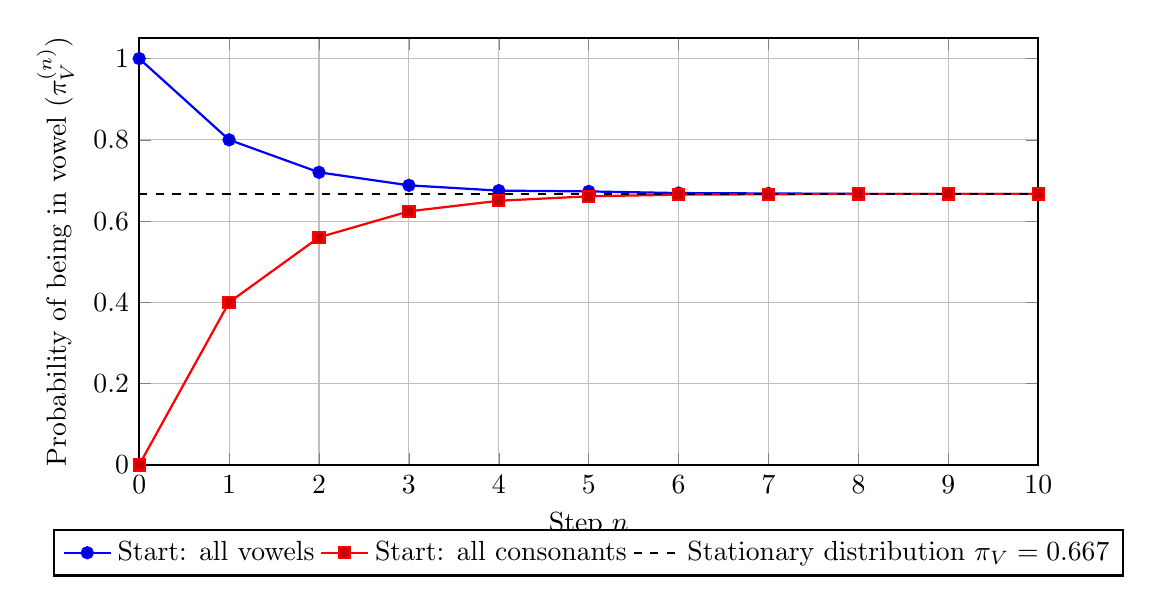
\begin{tikzpicture}
\begin{axis}[
    width=13cm, height=7cm,
    xlabel={Step $n$},
    ylabel={Probability of being in vowel ($\pi_V^{(n)}$)},
    xmin=0, xmax=10,
    ymin=0.0, ymax=1.05,
    grid=major,
    thick,
    legend style={at={(0.5,-0.15)}, anchor=north, legend columns=-1}
]

% Starting from all vowels
\addplot+[mark=*] coordinates {
(0, 1.000)
(1, 0.800)
(2, 0.720)
(3, 0.688)
(4, 0.675)
(5, 0.673)
(6, 0.669)
(7, 0.668)
(8, 0.667)
(9, 0.667)
(10, 0.667)
};
\addlegendentry{Start: all vowels}

% Starting from all consonants
\addplot+[mark=square*] coordinates {
(0, 0.000)
(1, 0.400)
(2, 0.560)
(3, 0.624)
(4, 0.650)
(5, 0.661)
(6, 0.665)
(7, 0.666)
(8, 0.667)
(9, 0.667)
(10, 0.667)
};
\addlegendentry{Start: all consonants}

% Stationary distribution line
\addplot[dashed, domain=0:10, samples=2] {0.667};
\addlegendentry{Stationary distribution $\pi_V = 0.667$}

\end{axis}
\end{tikzpicture}
\end{center}

\subsection*{Interpretation}

This plot shows how different initial starting conditions lead to the same long-run behavior.
Even though one chain begins entirely in vowels and the other entirely in consonants,
both converge to the same stationary distribution.
This illustrates the \emph{forgetting property} of Markov chains:
the system ``forgets'' its initial state and stabilizes in equilibrium.